
\begin{figure}[t]
     \centering
     \begin{subfigure}[b]{0.45\textwidth}
         \centering
         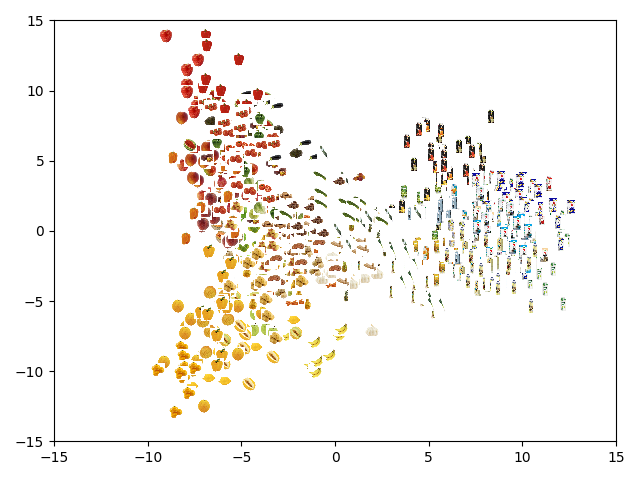
\includegraphics[width=\textwidth]{PaperB/figures_and_tables/latent_space_visualizations/splitae_vcca_comparison/pca_latents_splitae_xiwy_seed2.png}
         \caption{SplitAE$_{xiwy}$}
         \label{fig:splitae_xiwy_comparison}
     \end{subfigure}
     %\hfill
     \begin{subfigure}[b]{0.45\textwidth}
         \centering
         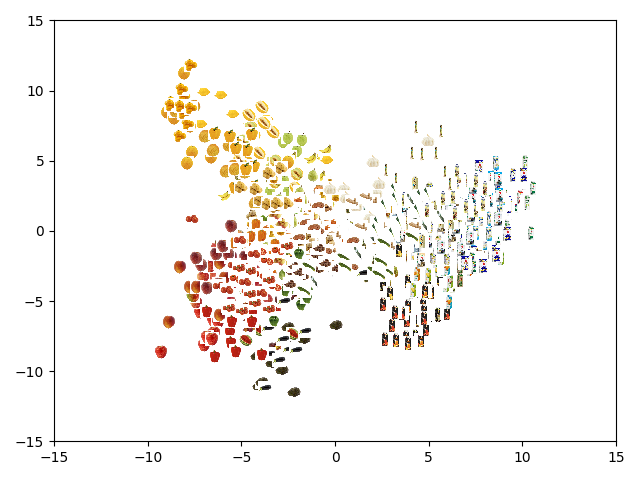
\includegraphics[width=\textwidth]{PaperB/figures_and_tables/latent_space_visualizations/splitae_vcca_comparison/pca_latents_vcca_xiwy_seed2.png}
         \caption{VCCA$_{xiwy}$}
         \label{fig:vcca_xiwy_comparison}
     \end{subfigure} \\
     %\hfill
     \begin{subfigure}[b]{0.45\textwidth}
         \centering
         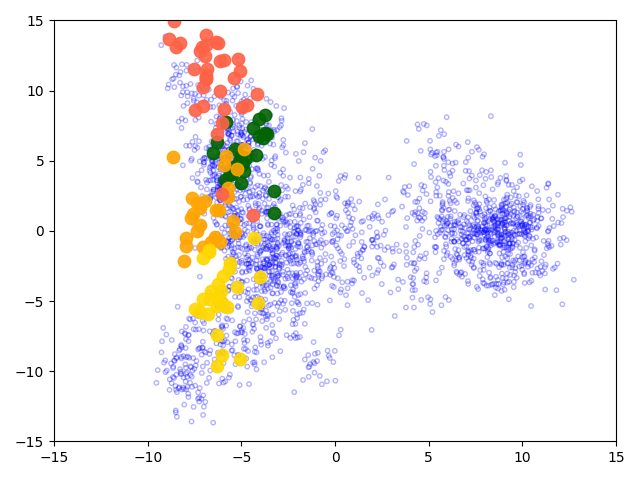
\includegraphics[width=\textwidth]{PaperB/figures_and_tables/latent_space_visualizations/splitae_vcca_comparison/pca_latent_peppers_splitae_xiwy_seed2.png}
         \caption{SplitAE$_{xiwy}$}
         \label{fig:splitae_xiwy_bell_peppers_comparison}
     \end{subfigure}
     \begin{subfigure}[b]{0.45\textwidth}
         \centering
         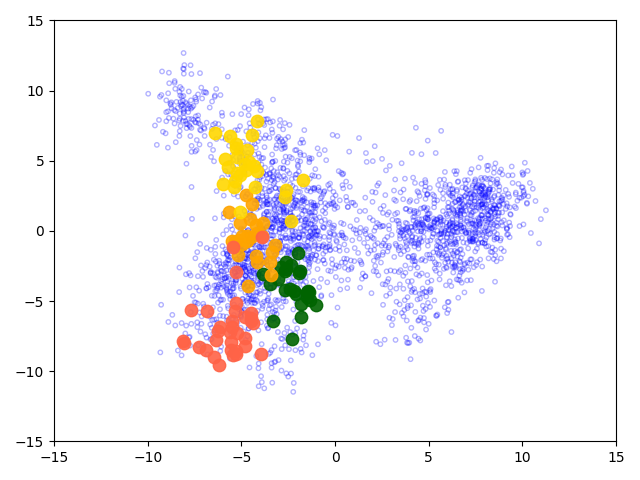
\includegraphics[width=\textwidth]{PaperB/figures_and_tables/latent_space_visualizations/splitae_vcca_comparison/pca_latent_peppers_vcca_xiwy_seed2.png}
         \caption{VCCA$_{xiwy}$}
         \label{fig:vcca_xiwy_bell_peppers_comparison}
     \end{subfigure}
        \caption{Visualizations of the latent representations of the test set from SplitAE$_{xiwy}$ and VCCA$_{xiwy}$. We plot the corresponding iconic image to each latent representation in Figure \ref{fig:splitae_xiwy_comparison} and \ref{fig:vcca_xiwy_comparison}. In Figure \ref{fig:splitae_xiwy_bell_peppers_comparison} and \ref{fig:vcca_xiwy_bell_peppers_comparison}, we plot the bell pepper representations according to the color of the class, while the blue points correspond to the other grocery items. Abbreviations: SplitAE, Split Autoencoder; VCCA, Variational Canonical Correlation Analysis.}
        \label{fig:2d_visualizations_pca_splitae_vcca_comparison}
\end{figure}